\documentclass{article}
\usepackage[hmargin=1.5in, vmargin=1in]{geometry}
\usepackage{amsmath}
\usepackage{amssymb}
\usepackage{graphicx}
\usepackage{tabularray}
\usepackage{fonttable}
\usepackage{minted}
\usepackage{tcolorbox}
\tcbuselibrary{listings, minted, breakable, skins}
\tcbset{listing engine=minted}
\definecolor{bg}{RGB}{242, 242, 242}
\setminted{
  fontsize=\small,
  bgcolor=bg
}
\DeclareTCBListing{code}{!O{tex}}{
  enhanced,
  breakable,
  colback=bg, 
  frame hidden, 
  left=1mm, right=1mm,
  top=0mm, bottom=0mm, 
  listing side text,
  minted language=#1, 
  minted style=manni,
  minted options = {  
    autogobble,
    tabsize=2,
    breaklines=true, 
    breakanywhere=true,
    breakanywheresymbolpre=,
    breaksymbolleft=,
    fontsize=\footnotesize
  }
}
\usepackage{hyperref}
\hypersetup{
  bookmarksnumbered,
  colorlinks = true,
  linkcolor = teal,
  urlcolor = red,
  citecolor = blue,
  pdfauthor = {Eureka},
  pdftitle = {LaTeX Hook Management Tutorial}
}

% font loading
\usepackage{amsfonts}
\DeclareMathAlphabet{\mathbf}{OT1}{cmr}{m}{sc}
\DeclareMathSymbol{\nsubseteq}{\mathrel}{AMSb}{"2A}
\DeclareMathSymbol{\myHbar}{\mathrel}{AMSb}{"7E}
\DeclareMathSymbol{\myDoublecup}{\mathbin}{AMSa}{"64}


\title{Font Config Notes}
\author{Eureka}
\date{\today}
\begin{document}
\maketitle
\tableofcontents
\newpage

\section{Text Font command}
Later we call the axis name by ``parameter'', then we call a font has 6 parameters.

\subsection{How to set font}
\begin{code}
-> code
\end{code}

\begin{code}
\fontencoding{T1}\fontfamily{cmss}\fontseries{bx}\fontshape{it}\selectfont
-> Hello world.
\end{code}

There is a short hand command \verb |\usefont|, equivalent to font set commands and a following selectfont command. An simple 
example as follows:
\begin{code}
\usefont{T1}{cmss}{bx}{it} 
-> Hello world.
\end{code}


\subsection{check the attributes of current font}
\begin{code}
\fontsize {12pt} {12pt}
\usefont{T1}{cmr}{m}{sc}
\makeatletter
Encoding = \f@encoding\par
Family = \f@family\par
Series = \f@series\par
Shape = \f@shape\par
Font size = \f@size\par
Baseline skip = \f@baselineskip

\vskip2em
\hskip-.5em\begin{tabular}[t]{lcl}
math size & = & value(pt) \\[.5em]
Main  & = & \(\tf@size\)\\
`script' & = & \(\sf@size\)\\
`scriptscript' & = & \(\ssf@size\)
\end{tabular}
\makeatother
\end{code}

The last three are accessible only within a formula; outside of math they may contain arbitrary values.

\subsection{set parameters}
Some default parameter values are:
\begin{code}
textrm = \rmdefault\par
textsf = \sfdefault\par
texttt = \ttdefault\par

\vskip1em
\textrm{Hello world.}\par 
\textsf{Hello world.}\par
\texttt{Hello world.}
\end{code}

What if we change it:
\begin{code}
\renewcommand{\rmdefault}{ptm}
\renewcommand{\sfdefault}{phv}
\renewcommand{\ttdefault}{pcr}

textrm = \rmdefault\par
textsf = \sfdefault\par
texttt = \ttdefault\par

\vskip1em
\textrm{Hello world.}\par 
\textsf{Hello world.}\par
\texttt{Hello world.}
\end{code}

The other default parameters values are:
\begin{code}
\encodingdefault\par
\familydefault\par
\seriesdefault\par
\shapedefault\par
\bfdefault\par
\mddefault\par
\itdefault\par
\sldefault\par
\scdefault\par
\sscdefault\par
\swdefault\par
\ulcdefault\par
\updefault
\end{code}

\subsection{Special font declaration commands}
Unlike the above \verb|\usefont|, there are some alternative commands to switch font:
\begin{itemize}
  \item \verb|\DeclareFixedFont|
  \item \verb|\DeclareTextFontCommand|: use syntax like \verb|<cmd>{ ... }|
  \item \verb|\DeclareOldFontCommand|: use syntax like \verb|{<cmd> ...}|
\end{itemize}



\section{Math Font command}
\subsection{math alphabets}
Math fonts called by \verb|\mathsf{}|, \verb|\mathbf{}| are called \textbf{math alphabets}(maybe 
called ``math letters (font)'' is better, in my opinion.), thus these math alphabet commands only affect:
\begin{itemize}
  \item fonts used for letters
  \item symbols of type \verb|\mathalpha|
\end{itemize}

\begin{code}
% default math rm font
\[\mathrm{Hello world}\]


% change the default text rm font
\renewcommand{\rmdefault}{ptm}
\[\mathrm{Hello world}\]
\end{code}


\subsection{math symbol fonts}
Some symbols font are called \textbf{math symbol fonts},  like the symbol \verb|\oplus|($\oplus$), \verb|>, +|($>, +$), these 
fonts that contain these symbols are called \textbf{math symbol fonts}.

\begin{center}
  \begin{tabular}{lcl}
    \hline
    Symbol font & Description & Example \\[.5em]
    \hline
    operators & symbols from \verb|\mathrm| & $[+]$ \\[.5em]
    letters   & symbols from \verb|\mathnormal|    & $<<\star>>$ \\[.5em]
    symbols   & most \LaTeX\ symbols        & $\le *\ge$ \\[.5em]
    largesymbols & large symbols            & $\sum\prod\int$ \\[.5em]
    \hline
  \end{tabular}
\end{center}

Like text font, Math fonts have the same 5 attributes, But don't have commands to change the attributes individually. 
To change these attributes, you should use \textbf{math version}, and this command change the whole attributes. There 
are 2 predefined math version:
\begin{itemize}
  \item normal: default, use \verb|\unboldmath| to select ``normal'' math version.
  \item bold : use command \verb|\boldmath| to select ``bold'' math version.
\end{itemize}

Or use command \verb|\mathversion{⟨version⟩}| to switch math version.

\begin{code}
\[ a^2 + b^2 = c^2 \]

\boldmath
\[ a^2 + b^2 = c^2 \]

\unboldmath
\[ a^2 + b^2 = c^2 \]
\end{code}


Use the External font attributes for math fonts in Text context. We use a font family named ``Computer Modern Math Symbols(cmsy)'',
The encoding is ``OMS''.
\begin{code}
\DeclareFixedFont{\textMathSwitch}{OMS}{cmsy}{m}{n}{10}
\textMathSwitch ABCXYZ

\DeclareFixedFont{\newtextMathSwitch}{OMS}{cmsy}{m}{n}{14}
\newtextMathSwitch ABCXYZ
\end{code}

There are \textbf{no commands} for selecting symbol fonts. Instead, these are selected
\textbf{indirectly} through symbol commands like \verb|\oplus|.

\subsection{Declaring math versions}
We can declare math font (cmd) version by \verb|\DeclareMathVersion|. Unlike the text font command that can change 
a single parameter value, the math version command need to change the whole parameters based on the math version declared so far.



\subsection{Declaring math alphabets}
An example to change the default math alphabets font:

\begin{code}
% this declaration should be in preamble
% \DeclareMathAlphabet{\mathbf}{OT1}{cmr}{m}{sc}
\[ \mathbf{Hello World} \]
\end{code}

You can use \verb|\SetMathAlphabet| to set math alphabet for a specific math version or 
\textbf{fixed the defined nowhere error caused by no shape}.


\subsection{Declaring symbol fonts}
Just copy some example from the the doc: For example, the following sets up the first four standard math symbol fonts:
\begin{verbatim}
\DeclareSymbolFont{operators}{OT1}{cmr}{m}{n}
\DeclareSymbolFont{letters}{OML}{cmm}{m}{it}
\DeclareSymbolFont{symbols}{OMS}{cmsy}{m}{n}
\DeclareSymbolFont{largesymbols}{OMX}{cmex}{m}{n}
\end{verbatim}

You can declare a new symbols font like the following (refer to TeX-SE:Difficulty in using slot to declare math symbol):
\begin{verbatim}
\@ifundefined{mathbb}{%
  \DeclareSymbolFontAlphabet{\mathbb}{AMSb}%
}{}
\DeclareSymbolFont{AMSb}{U}{msb}{m}{n}
\DeclareMathAlphabet{\mathbb}{U}{msb}{m}{n}
\end{verbatim}

Then you can define your own math symbols using the new symbols font.

\subsection{Declaring math symbols}
This is the most interesting part to me. Let's see how it works:\\
\textbullet\ \verb|\DeclareMathSymbol {⟨symbol⟩} {⟨type⟩} {⟨sym-font⟩} {⟨slot⟩}|

The \verb|⟨symbol⟩| can be:
\begin{itemize}
  \item a single character, like \verb|>|
  \item a control sequence, like \verb|\sum|
\end{itemize}

The \verb|⟨type⟩| is as follows:
\begin{center}
  \begin{tabular}{ccc}
    \hline
    \emph{Type} & \emph{Meaning} & \emph{Example} \\[.5em]
    \hline
    0 or \verb|\mathord  | & Ordinary           & $\alpha$ \\[.5em]
    1 or \verb|\mathop   | & Large operator     & $\sum$ \\[.5em]
    2 or \verb|\mathbin  | & Binary operation   & $\times$ \\[.5em]
    3 or \verb|\mathrel  | & Relation           & $\leq$ \\[.5em]
    4 or \verb|\mathopen | & Opening            & $\langle$ \\[.5em]
    5 or \verb|\mathclose| & Closing            & $\rangle$ \\[.5em]
    6 or \verb|\mathpunct| & Punctuation        & $;$ \\[.5em]
    7 or \verb|\mathalpha| & Alphabet character & $A$ \\[.5em]
    \hline
  \end{tabular}
\end{center}

Some inner symbols definition:
\begin{verbatim}
\DeclareMathSymbol{\alpha}{0}{letters}{"0B}
\DeclareMathSymbol{\lessdot}{\mathbin}{AMSb}{"0C}
\DeclareMathSymbol{\alphld}{\mathalpha}{AMSb}{"0C}
\end{verbatim}

What is \texttt{AMSb} symbols font ? In the previous, there are only 4 symbol fonts: operators, letters, symbols, largesymbols.
And what is \verb|⟨slot⟩| ? Is this something like glyph index ? And how to extract slot from the font tabel ? 
There is an original definition for \verb|\nsubseteq| from document ``User's Guide to AMSFonts Version 2.2d'':

\begin{code}
% can be only used in preamble
% \usepackage{amsfonts}
% \DeclareMathSymbol{\nsubseteq}{\mathrel}{AMSb}{"2A}
\[ \nsubseteq \]
\end{code}

You can setup your own math symbols font, do not forget to load package \verb|amsfonts|(and \texttt{amssymb} is superset of 
the \texttt{amsfonts} package,) in your preamble.

\begin{code}
% can be only used in preamble
% \usepackage{amsfonts}
% \DeclareMathSymbol{\myHbar}{\mathrel}{AMSb}{"7E}
\[ \myHbar \]

% \DeclareMathSymbol{\myDoublecup}{\mathbin}{AMSa}{"64}
\[ \myDoublecup \]
\end{code}

The ``slot'' can be found in document ``User's Guide to AMSFonts Version 2.2d''. The tables for symbols font look like:

\begin{figure}[!htb]
  \centering
  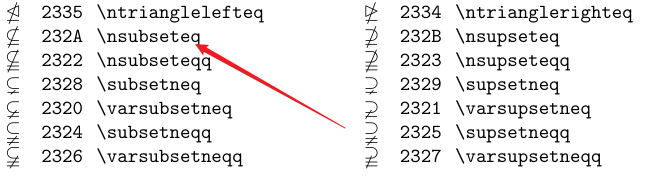
\includegraphics[width=.75\linewidth]{symbols_font_table_I.png}
  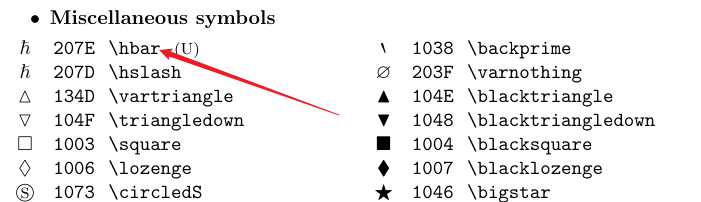
\includegraphics[width=.75\linewidth]{symbols_font_table_II.png}
  \caption{symbols font table in AMS fonts}
  \label{fig:ams-symbols-font-table}
\end{figure}

We just need to find the last 2 digits of the index as a slot number in \verb|\DeclareMathSymbol|, this is so easy. The document has 
already said the digits meaning in these table:
\begin{itemize}
  \item First digit identifies font: `1-AMSa', `2-AMSb'
  \item Second digit identifies class: `0-mathord', `2-mathbin', `3-mathrel'
  \item Third and fourth digits identify \textbf{(hex) location} in font
\end{itemize}

Thus it is true that the last 2 digits of the index are the slot number in the font table. The fisrt
digit already used when we declare the symbol font. Such as the `AMSb'(the first digit is 2) in \verb|\myHbar| definition;
The `AMSa'(the fisrt digit is 1), the `\verb|\mathbin|'(the Second digit is 2) in \verb|\mysquigarrow| definition.


\subsection{Declaring math sizes}


\subsection{Mind map for math font}


\section{Font table}
\subsection{introduction}
\begin{itemize}
  \item How to find your symbols for a given font, such as the default ``cmr10''? 
  \item How to see all avaliable symbols(glyphs) for a given font ? 
  \item What are \verb|\char, \chardef| doing for us?
\end{itemize}


\subsection{see font table}
We first show how to see all the avaliable symbols for a given font, such as the default ``cmr10''. There are 2 ways:
\begin{itemize}
  \item use package \verb|fonttable| in preamble
  \item type \verb|pdftex testfont| in shell 
\end{itemize}

The first method use example:
\begin{minted}{latex}
\documentclass{article}
\usepackage{fonttable}
\begin{document}
\fonttable{cmr10}
\end{document}
\end{minted}
Then you will get a font table like Table 1:

\fonttable{cmr10}
\centerline{Table 1: Computer modern roman 10 font table}
\stepcounter{table}
\vskip1em

Use this package, the \textbf{slot}(decimal) is automatically shown in the table.

The second method is type the font table in shell, the red content is what you need to type:
\begin{minted}[escapeinside=||]{text}
$ pdftex testfont
This is pdfTeX, Version 3.141592653-2.6-1.40.26 (TeX Live 2024) (preloaded format=pdftex)
  restricted \write18 enabled.
entering extended mode
(c:/texlive/2024/texmf-dist/tex/plain/knuth-lib/testfont.tex

Name of the font to test = |\color{red}cmsy10|
Now type a test command (\help for help):)
*|\color{red}\string\table|

*|\color{red}\string\bye|
[1{c:/texlive/2024/texmf-var/fonts/map/pdftex/updmap/pdftex.map}]<c:/texlive/20
24/texmf-dist/fonts/type1/public/amsfonts/cm/cmr10.pfb><c:/texlive/2024/texmf-d
ist/fonts/type1/public/amsfonts/cm/cmr7.pfb><c:/texlive/2024/texmf-dist/fonts/t
ype1/public/amsfonts/cm/cmsy10.pfb><c:/texlive/2024/texmf-dist/fonts/type1/publ
ic/amsfonts/cm/cmti10.pfb><c:/texlive/2024/texmf-dist/fonts/type1/public/amsfon
ts/cm/cmtt10.pfb>
Output written on testfont.pdf (1 page, 72741 bytes).
Transcript written on testfont.log.
\end{minted}

You will get something like table \ref{fig:cmsy10-font-table}:
\begin{table}[!htb]
  \centering
  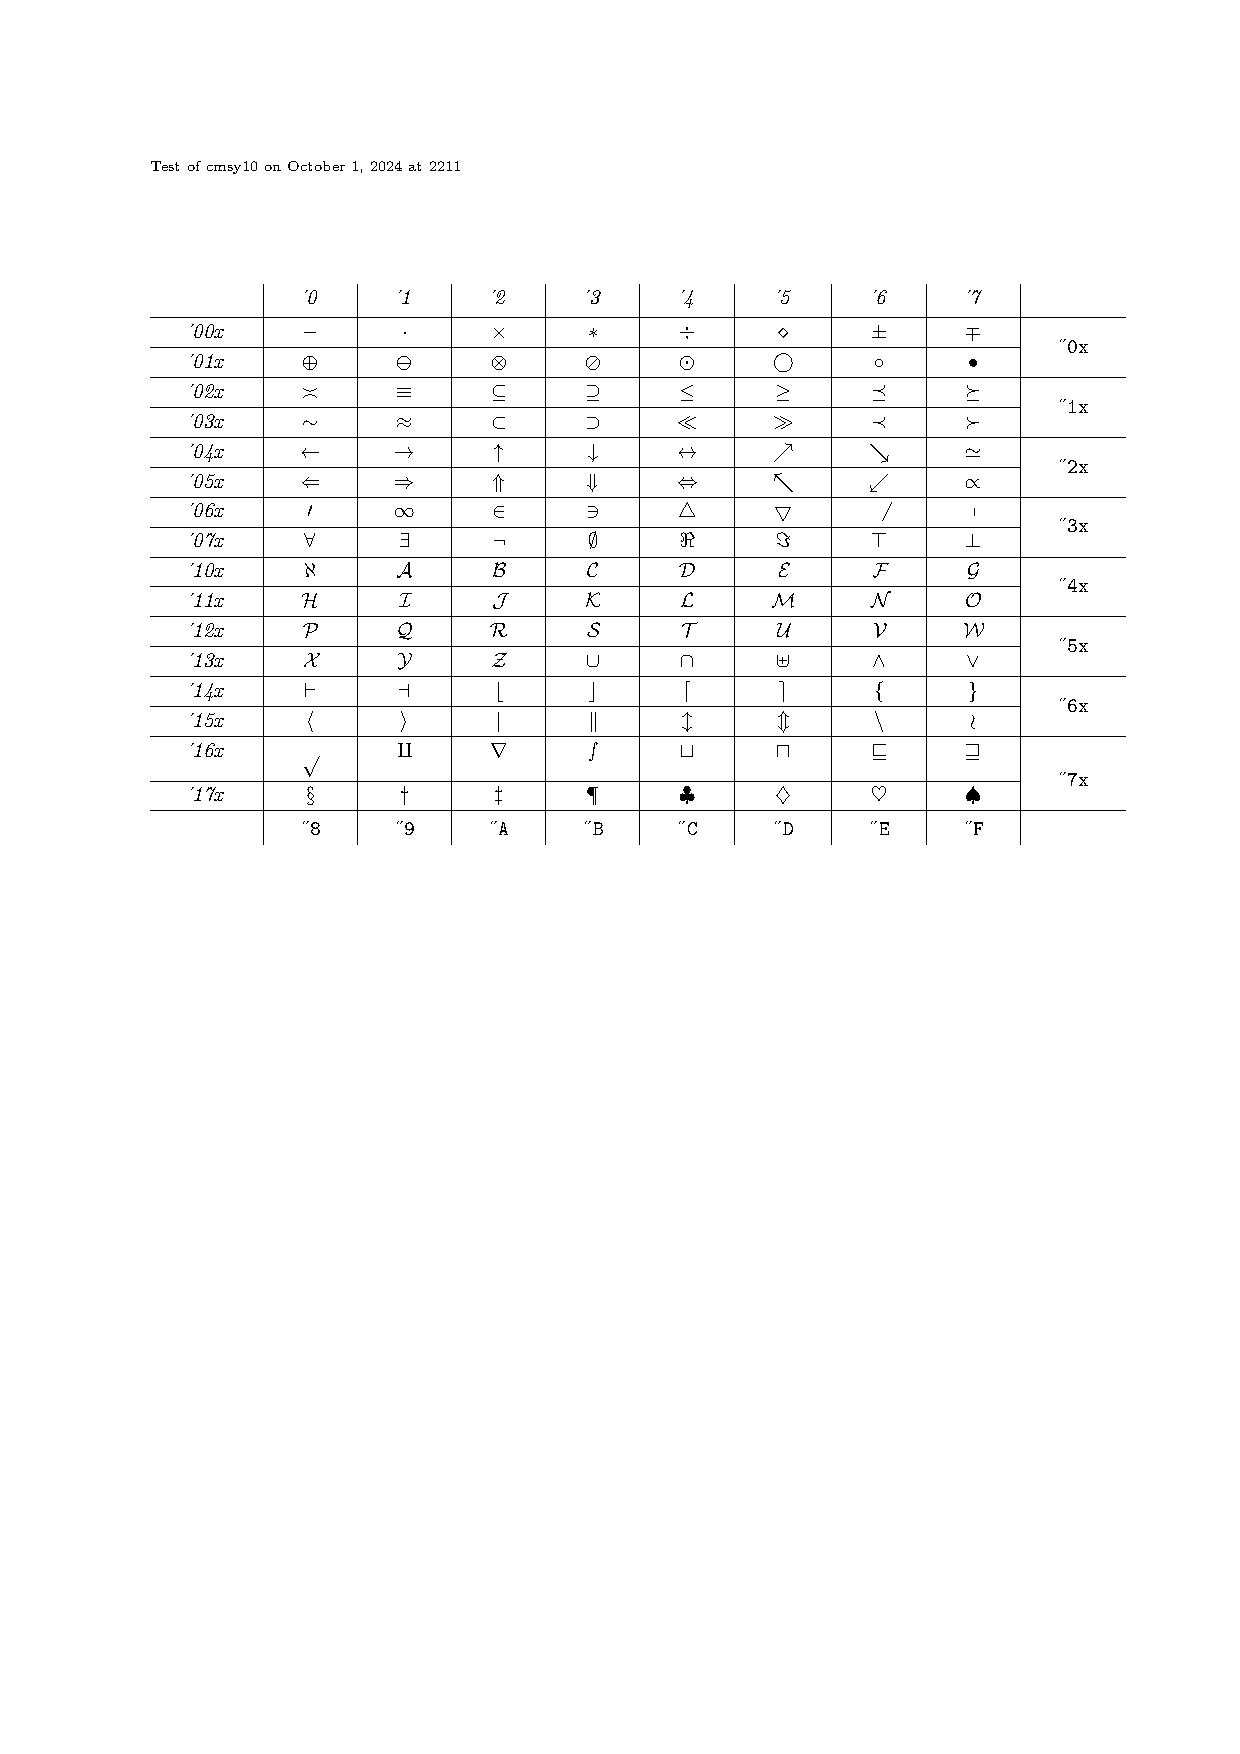
\includegraphics[width=.8\linewidth]{cmsy10_font_table.pdf}
  \caption{cmsy10 font table}
  \label{fig:cmsy10-font-table}
\end{table}

Whilst, there is no slot number in the table this time. Another font table(cmex) for Large symbol font:
\begin{table}[!htb]
  \centering
  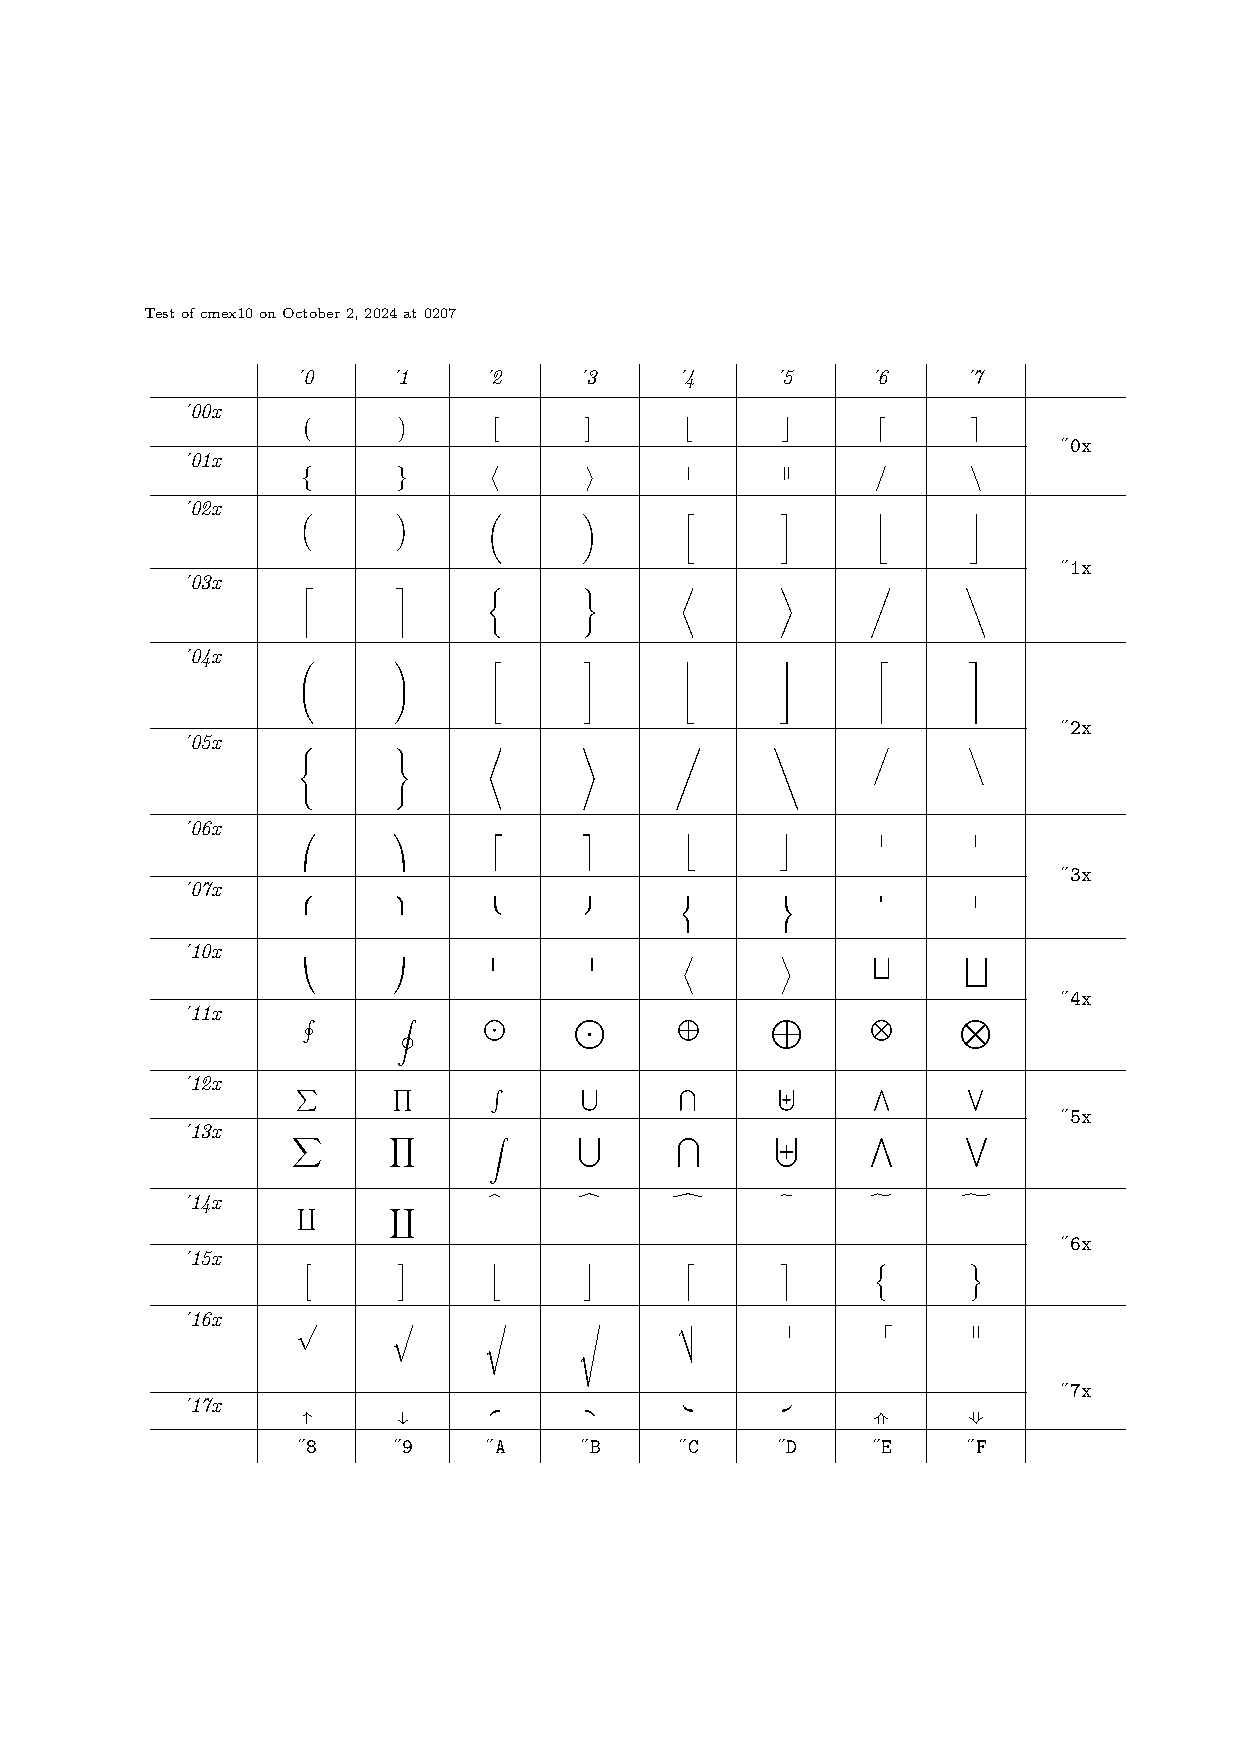
\includegraphics[width=.8\linewidth]{cmex10_font_table.pdf}
  \caption{cmsy10 font table}
  \label{fig:cmex10-font-table}
\end{table}


\subsection{\texttt{\protect\string\char} command}
How to type the symbols(glyphs) in the above font table? There are 2 ``coordinate" systems:
\begin{itemize}
  \item left and upper: the \textbf{octal} number coordinate
  \item right and lower: the \textbf{hex} number coordinate
\end{itemize}

For example, if we want to type the \textbf{dollar} character: ``\$'', there are two ways:
\begin{code}
% octal
Octal number: \char'044

% hex 
Hex number: \char"24\char"2C

% slot
Slot(decimal) number: \char36

% \chardef 
\chardef\mydollar=36
Chardef Command: \mydollar
\end{code}

The \texttt{'x'} in \texttt{`04x} means the `x' coordinate, in this case, it is `\texttt{`4}'. For hex coordinate, this is
a little different. Each hex row consists of 2 rows, in this case, the first row is from `\texttt{"20}' to `\texttt{"27}', the second 
row is from `\texttt{"28}' to `\texttt{"2f}'. In both case we have 
\[
  044\text{octal} = 24\text{hex} = 36\text{decimal}
\]

\textbf{Remark}: the \texttt{'} represents the octal number, and the \texttt{"} represents the hex number, and 
\texttt{`} represents the decimal(slot) number.

\subsection{\texttt{\protect\string\mathcal} for lowercase}
If you type lowercase letters in command \verb|\mathcal|, you will get a wrong result, only upper case letters, like \verb|\mathcal{A}|
will get the right script font. 

This for that \verb|\mathcal{<char>}| will use the slot number in the font table; Take letter `A' for example, the slot number is ``65'',
In the font table, slot number ``65(decimal)'' is just the script style `A'. Whilst, the slot number for `a' is ``97('141 in octal)'', and the 
result is a orthogonal symbol.

\begin{code}
% \usepackage{amsmath}
\begin{align}
  & \mathcal{A} \\
  & \mathcal{a}
\end{align}
\end{code}
\end{document}